\chapter{Methodology}
\label{ch:methodology}

This chapter presents the complete design of the proposed Hierarchical Federated Learning framework for traffic flow prediction. The framework operates in two phases: an offline \textit{clustering phase} that partitions the sensor network by temporal pattern similarity using Dynamic Time Warping, and an online \textit{federated training phase} that performs two-level aggregation with adaptive client selection. Figure~\ref{fig:framework_overview} provides a high-level overview of the pipeline.

\begin{figure}[htbp]
\centering
\includegraphics[width=\textwidth]{figures/framework_overview.png}
\caption{Overview of the proposed Hierarchical Federated Learning framework.}
\label{fig:framework_overview}
\end{figure}

\section{Problem Formulation}
\label{sec:problem}

Consider a traffic sensor network consisting of $N$ sensors deployed across a metropolitan road network. Each sensor $i \in \{1, \dots, N\}$ records traffic speed measurements at regular 5-minute intervals. Let $\mathbf{x}_i^{(t)} \in \mathbb{R}$ denote the speed reading of sensor $i$ at time step $t$.

\textbf{Traffic Flow Prediction Task.} Given a historical observation window of $L$ time steps, the goal is to predict the next $H$ time steps:
\begin{equation}
\label{eq:prediction_task}
\hat{\mathbf{y}}_i = f_{\theta_i}\left(\mathbf{x}_i^{(t-L+1)}, \mathbf{x}_i^{(t-L+2)}, \dots, \mathbf{x}_i^{(t)}\right) \in \mathbb{R}^H
\end{equation}
where $f_{\theta_i}$ is a parameterized prediction model for sensor $i$, $L = 12$ (1 hour of history), and $H = 12$ (1 hour forecast horizon). Following the METR-LA benchmark convention \cite{li2018}, predictions are evaluated at three horizons: 15 minutes ($h=3$), 30 minutes ($h=6$), and 60 minutes ($h=12$).

\textbf{Federated Learning Formulation.} In the federated setting, each sensor $i$ holds a private local dataset $\mathcal{D}_i = \{(\mathbf{X}_i^{(k)}, \mathbf{y}_i^{(k)})\}_{k=1}^{n_i}$ of sliding-window input--output pairs. The raw data $\mathcal{D}_i$ never leaves the edge device. The objective is to collaboratively learn model parameters that minimize the weighted empirical risk across all sensors \cite{mcmahan2017}:
\begin{equation}
\label{eq:fl_objective}
\min_{\theta} \quad F(\theta) = \sum_{i=1}^{N} \frac{n_i}{\sum_{j} n_j} \cdot \mathcal{L}_i(\theta; \mathcal{D}_i)
\end{equation}
where $\mathcal{L}_i$ is the local loss function (Mean Squared Error) for sensor $i$.

However, the standard FedAvg solution to Equation~\ref{eq:fl_objective} assumes data across clients is approximately IID. In traffic networks, this assumption is strongly violated: highway sensors observe high-speed, low-variance patterns while urban intersection sensors exhibit stop-and-go dynamics. This \textit{statistical heterogeneity} motivates the clustered approach described in the following sections.

\section{Theoretical Foundations}
\label{sec:foundations}

This section briefly summarizes the theoretical concepts underlying the proposed framework. Detailed equations for each component are provided in their respective implementation sections.

\subsection{Federated Learning}
\label{sec:fl_theory}

Federated Learning (FL) is a distributed machine learning paradigm introduced by McMahan et al. \cite{mcmahan2017} that enables multiple clients to collaboratively train a shared model without exchanging raw data \cite{kairouz2021}. The foundational algorithm, \textit{Federated Averaging} (FedAvg), operates in iterative communication rounds: the server broadcasts the current model to selected clients, each client performs multiple local optimization steps on its private data, and the server aggregates the updated models via weighted averaging (see Section~\ref{sec:fl_framework} for the formal protocol). The key insight of FedAvg is that performing multiple local steps before aggregation significantly reduces the number of communication rounds, making it practical for bandwidth-constrained edge networks \cite{konecny2016}. However, each round still incurs a communication cost proportional to the model size, which reaches tens of gigabytes in the experiments reported in this thesis (Section~\ref{sec:comm_cost}).

\subsection{Gated Recurrent Units and Sequence-to-Sequence Models}
\label{sec:gru_theory}

Traffic flow prediction requires models that capture temporal dependencies across sequential observations. Standard Recurrent Neural Networks (RNNs) suffer from the \textit{vanishing gradient problem} \cite{hochreiter1997}: gradients shrink exponentially with sequence length during backpropagation through time, preventing the network from learning long-range dependencies.

The Gated Recurrent Unit (GRU) \cite{cho2014} addresses this through \textit{gating mechanisms}, an update gate and a reset gate, that control information flow and create identity shortcuts for gradient propagation. When the update gate is near zero, the hidden state passes through unchanged, allowing the network to retain information across many time steps. The full GRU equations are provided in Section~\ref{sec:model}.

For multi-step forecasting, the \textit{Encoder-Decoder} (Sequence-to-Sequence) architecture \cite{cho2014} extends single-step prediction to arbitrary output lengths. The encoder compresses the input sequence into a fixed-size context vector, and the decoder generates predictions autoregressively; each predicted value is fed as input to produce the next (Section~\ref{sec:model}). This naturally handles the mapping from a 1-hour historical window to a 1-hour future prediction.

\subsection{Non-IID Data in Traffic Networks}
\label{sec:noniid_theory}

A fundamental assumption of FedAvg is that data across clients is \textit{Independent and Identically Distributed} (IID). In traffic networks, this assumption is strongly violated through three mechanisms:

\begin{itemize}
    \item \textbf{Feature Distribution Skew:} Highway sensors record speeds around 60--70 mph with low variance, while arterial sensors exhibit bimodal distributions (congested vs. free flow).
    \item \textbf{Temporal Pattern Heterogeneity:} Rush-hour timing and incident responses vary by location, creating phase-shifted patterns that DTW can capture but Euclidean distance cannot.
    \item \textbf{Concept Drift:} Long-term changes (road construction, new signals) affect sensors differently, shifting local distributions over time.
\end{itemize}

When FedAvg is applied naively to such heterogeneous data, \textit{client drift} occurs \cite{zhao2018, karimireddy2020}: each client's local updates push the model toward its own distribution, and averaging these divergent updates produces a model that fits no distribution well. The clustered approach adopted in this thesis mitigates client drift by ensuring sensors within each cluster share similar temporal patterns, making intra-cluster data more statistically homogeneous and reducing client drift.

\section{Dataset and Preprocessing}
\label{sec:dataset}

\subsection{METR-LA Dataset}
The experiments use the METR-LA (Metropolitan Traffic --- Los Angeles) dataset \cite{li2018}, a widely used benchmark for traffic forecasting research. The dataset contains speed readings from $N = 207$ loop-detector sensors deployed across the Los Angeles highway network, recorded at 5-minute intervals over 4 months (March--June 2012). This yields approximately 34,272 time steps per sensor.

\subsection{Zero-Speed Masking and Imputation}
\label{sec:zero_masking}
A critical preprocessing step involves handling zero-valued speed readings. In the METR-LA dataset, $0.0$ mph readings are treated as sensor failures or missing measurements rather than reliable traffic observations. Approximately 8.11\% of all readings are zeros.

Treating these as valid observations corrupts normalization statistics and introduces artificial patterns. The preprocessing pipeline therefore:
\begin{enumerate}
    \item Replaces all $0.0$ readings with $\texttt{NaN}$ to mark them as missing.
    \item Imputes each missing value with the \textit{per-sensor temporal mean}:
    \begin{equation}
    x_i^{(t)} \leftarrow \bar{x}_i = \frac{1}{|\mathcal{T}_i^{\text{valid}}|} \sum_{t' \in \mathcal{T}_i^{\text{valid}}} x_i^{(t')}
    \end{equation}
    where $\mathcal{T}_i^{\text{valid}}$ is the set of non-zero time steps for sensor $i$.
\end{enumerate}

\subsection{Normalization}
After imputation, each sensor's time series is independently standardized using z-score normalization, following the preprocessing convention of Li et al. \cite{li2018}:
\begin{equation}
\tilde{x}_i^{(t)} = \frac{x_i^{(t)} - \mu_i}{\sigma_i}
\end{equation}
where $\mu_i$ and $\sigma_i$ are the mean and standard deviation of sensor $i$'s training data. Predictions are denormalized before evaluation to compute metrics in original speed units (mph).

\subsection{Sliding Window Construction}
The normalized time series is divided into supervised input--output pairs using a sliding window approach \cite{li2018}:
\begin{equation}
\mathbf{X}^{(k)} = [\tilde{x}^{(k)}, \tilde{x}^{(k+1)}, \dots, \tilde{x}^{(k+L-1)}], \quad
\mathbf{y}^{(k)} = [\tilde{x}^{(k+L)}, \dots, \tilde{x}^{(k+L+H-1)}]
\end{equation}
where $L = 12$ and $H = 12$. The dataset is split chronologically (no shuffling) into 70\% training, 10\% validation, and 20\% test sets.

\subsection{Time-of-Day Features}
\label{sec:tod_features}
Traffic patterns exhibit strong diurnal periodicity. To enable the model to leverage this, the framework optionally augments input features using a sinusoidal cyclical encoding inspired by positional encodings \cite{vaswani2017attention}. For each time step $t$ with 5-minute interval index $d_t \in \{0, 1, \dots, 287\}$ (where $288 = 24 \times 12$):
\begin{equation}
\text{sin\_tod}_t = \sin\left(\frac{2\pi \cdot d_t}{288}\right), \quad
\text{cos\_tod}_t = \cos\left(\frac{2\pi \cdot d_t}{288}\right)
\end{equation}
This maps the discrete time index to a continuous representation on the unit circle, ensuring that 23:55 and 00:00 are neighbors in feature space. When enabled, the input feature vector becomes $[\tilde{x}_i^{(t)}, \sin\_\text{tod}_t, \cos\_\text{tod}_t] \in \mathbb{R}^3$.

\section{DTW-Based Traffic Pattern Clustering}
\label{sec:dtw_clustering}

\subsection{Motivation}
Standard approaches to partitioning sensor networks for federated learning rely on graph topology (e.g., spectral clustering of the adjacency matrix). However, topologically adjacent sensors can exhibit vastly different traffic dynamics---for instance, a highway on-ramp and the adjacent off-ramp display opposite flow patterns during rush hours. This thesis adopts Dynamic Time Warping (DTW) to cluster sensors by \textit{temporal pattern similarity}, following Feng et al. \cite{feng2024}.

\subsection{Dynamic Time Warping Distance}
Given two time series $\mathbf{s}_i = (s_i^1, \dots, s_i^T)$ and $\mathbf{s}_j = (s_j^1, \dots, s_j^T)$ of length $T$, DTW finds the optimal alignment between them by computing the cumulative cost matrix $D \in \mathbb{R}^{(T+1) \times (T+1)}$ via dynamic programming \cite{sakoe1978}:
\begin{equation}
\label{eq:dtw}
D(a, b) = |s_i^a - s_j^b| + \min\begin{cases} D(a-1, b) \\ D(a, b-1) \\ D(a-1, b-1) \end{cases}
\end{equation}
with boundary condition $D(0, 0) = 0$ and $D(a, 0) = D(0, b) = \infty$ for $a, b > 0$. The DTW distance is $\text{DTW}(\mathbf{s}_i, \mathbf{s}_j) = D(T, T)$. Unlike Euclidean distance, DTW handles phase shifts in periodic traffic patterns (e.g., rush hour starting 15 minutes earlier at one sensor versus another).

\subsection{Clustering Pipeline}
The clustering pipeline proceeds in four steps:

\textbf{Step 1: Representative Series Extraction.} For each sensor $i$, a representative time series of length $T_s = 300$ is extracted from the first timestep of each training window. Each series is independently z-score normalized to ensure DTW measures \textit{shape similarity} rather than absolute scale:
\begin{equation}
\bar{s}_i^{(t)} = \frac{s_i^{(t)} - \mu_{s_i}}{\sigma_{s_i} + \epsilon}, \quad \epsilon = 10^{-8}
\end{equation}

\textbf{Step 2: Pairwise DTW Distance Matrix.} The full $N \times N$ pairwise distance matrix $\mathbf{M}$ is computed, where $M_{ij} = \text{DTW}(\bar{\mathbf{s}}_i, \bar{\mathbf{s}}_j)$. For $N = 207$ sensors and $T_s = 300$, this requires $\binom{207}{2} = 21{,}321$ DTW computations, taking approximately 3--5 minutes on CPU.

\textbf{Step 3: Classical MDS Embedding.} Since K-Means requires Euclidean input, the DTW distance matrix is embedded into Euclidean space via Classical Multidimensional Scaling (MDS) \cite{cox2000}. The top $d = \min(2K, N-1)$ eigenvectors of the double-centered squared distance matrix are retained, mapping each sensor to a $d$-dimensional coordinate suitable for Euclidean clustering.

\textbf{Step 4: K-Means Clustering.} K-Means \cite{macqueen1967} with $K = 8$ clusters and 10 random initializations is applied to the MDS embedding. The resulting labels $\{c_1, \dots, c_N\}$ partition sensors into $K$ groups with similar temporal traffic dynamics.

\subsection{Selection of $K$}
The number of clusters was determined using a combination of statistical analysis and domain considerations. Figure~\ref{fig:k_selection} shows the within-cluster inertia (elbow method) and silhouette score for $K = 2$ to $15$. While the silhouette score is maximized at $K = 2$ and the elbow inflection occurs around $K = 3$, these coarse partitions are insufficient for traffic applications: they capture only the broadest distinction (e.g., highway vs. arterial) and merge sensors with fundamentally different congestion dynamics. $K = 8$ was selected as a practical tradeoff---it lies in the region of diminishing inertia returns while providing meaningful traffic granularity (separating rush-hour-dominated sensors from steady-flow and ramp sensors). Importantly, the smallest cluster contains 8 sensors (see the per-cluster breakdown in Table~\ref{tab:cluster_results}), ensuring sufficient data diversity for effective intra-cluster federated averaging. $K = 8$ should therefore be interpreted as a domain-motivated design choice rather than the statistically optimal cluster count.

\begin{figure}[htbp]
\centering
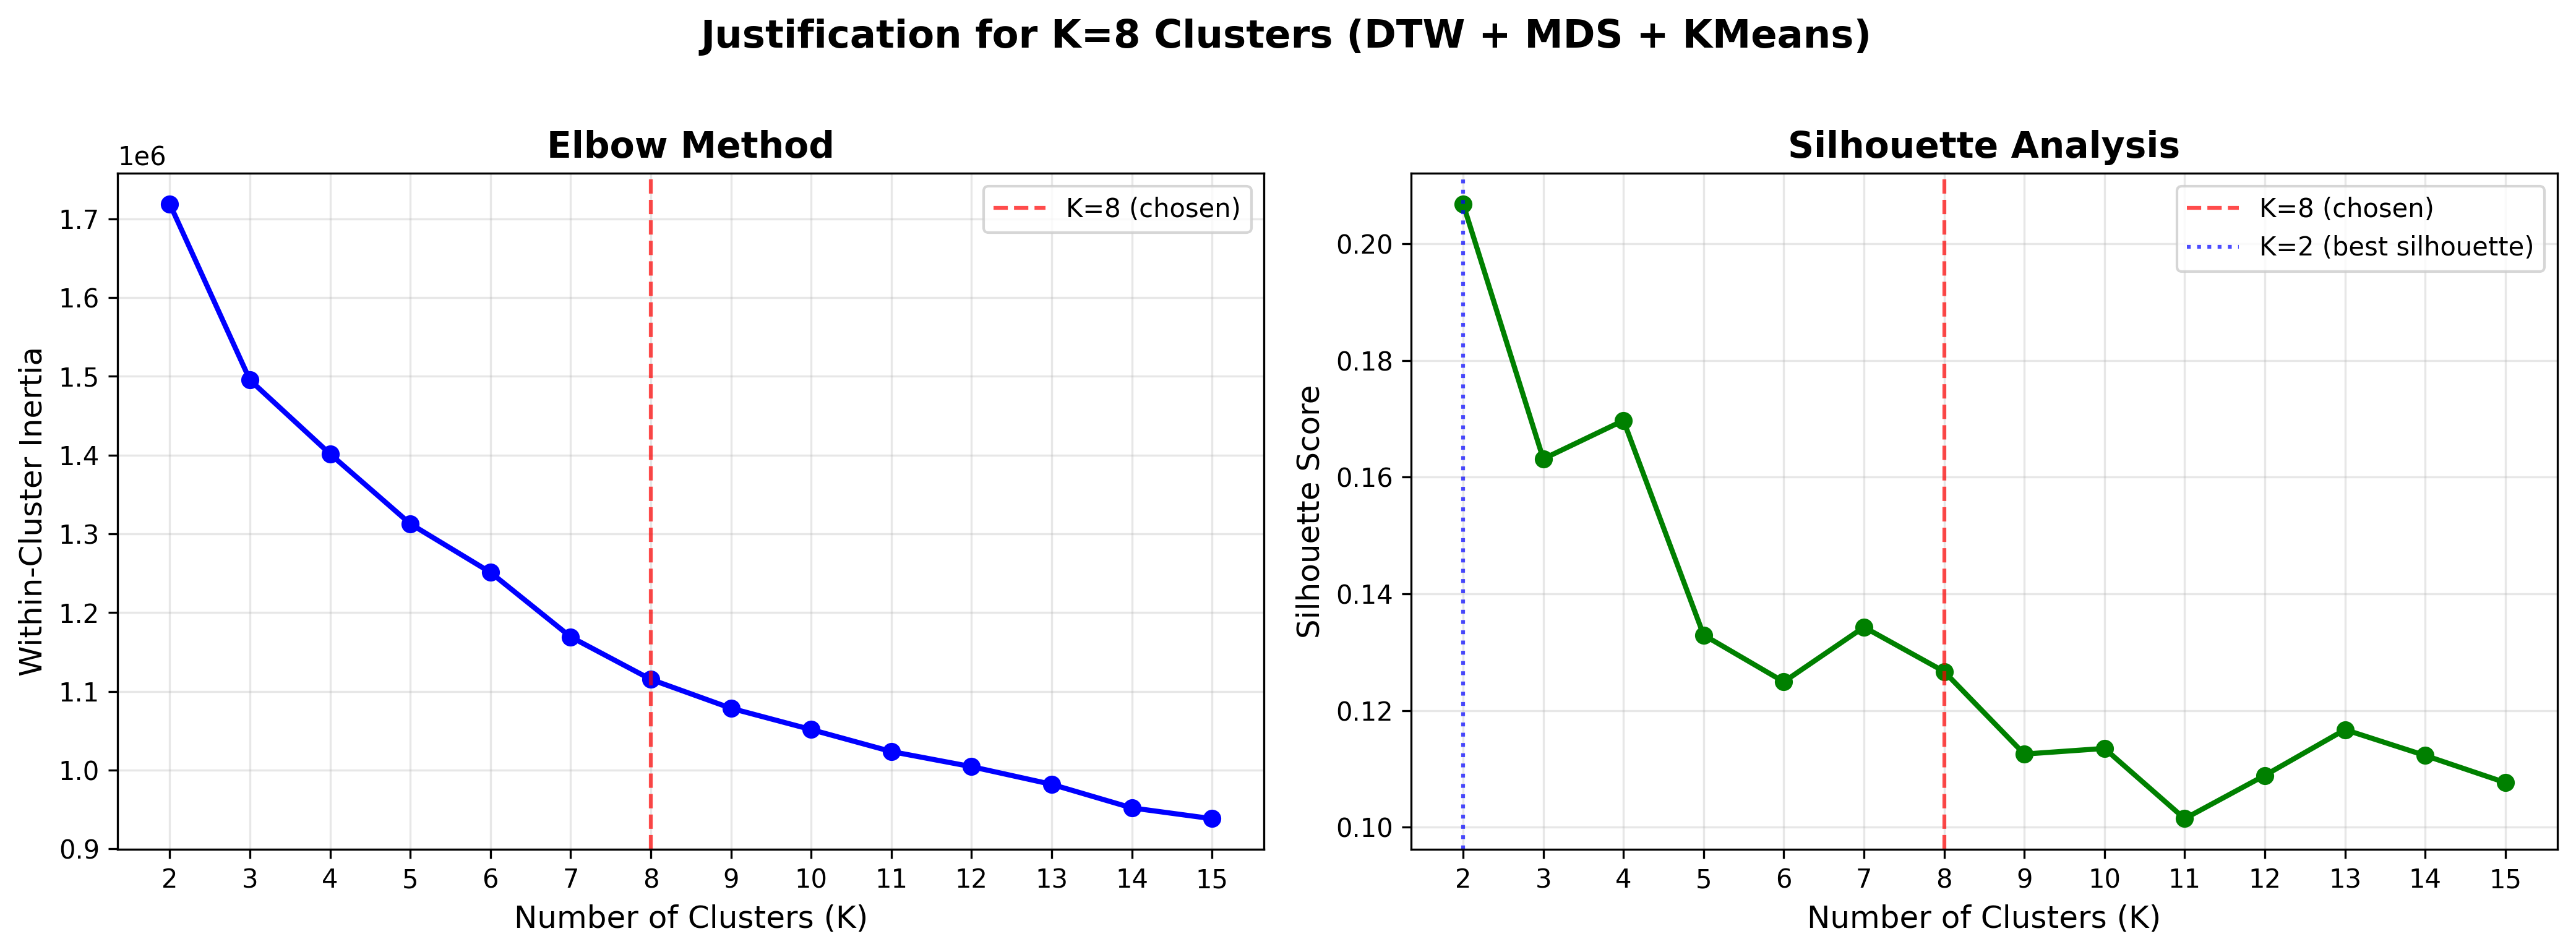
\includegraphics[width=\textwidth]{figures/k_selection_analysis.png}
\caption{Cluster selection analysis. Left: within-cluster inertia vs. $K$ (elbow method). Right: silhouette score vs. $K$. The dashed red line indicates the chosen $K = 8$.}
\label{fig:k_selection}
\end{figure}

\begin{figure}[htbp]
\centering
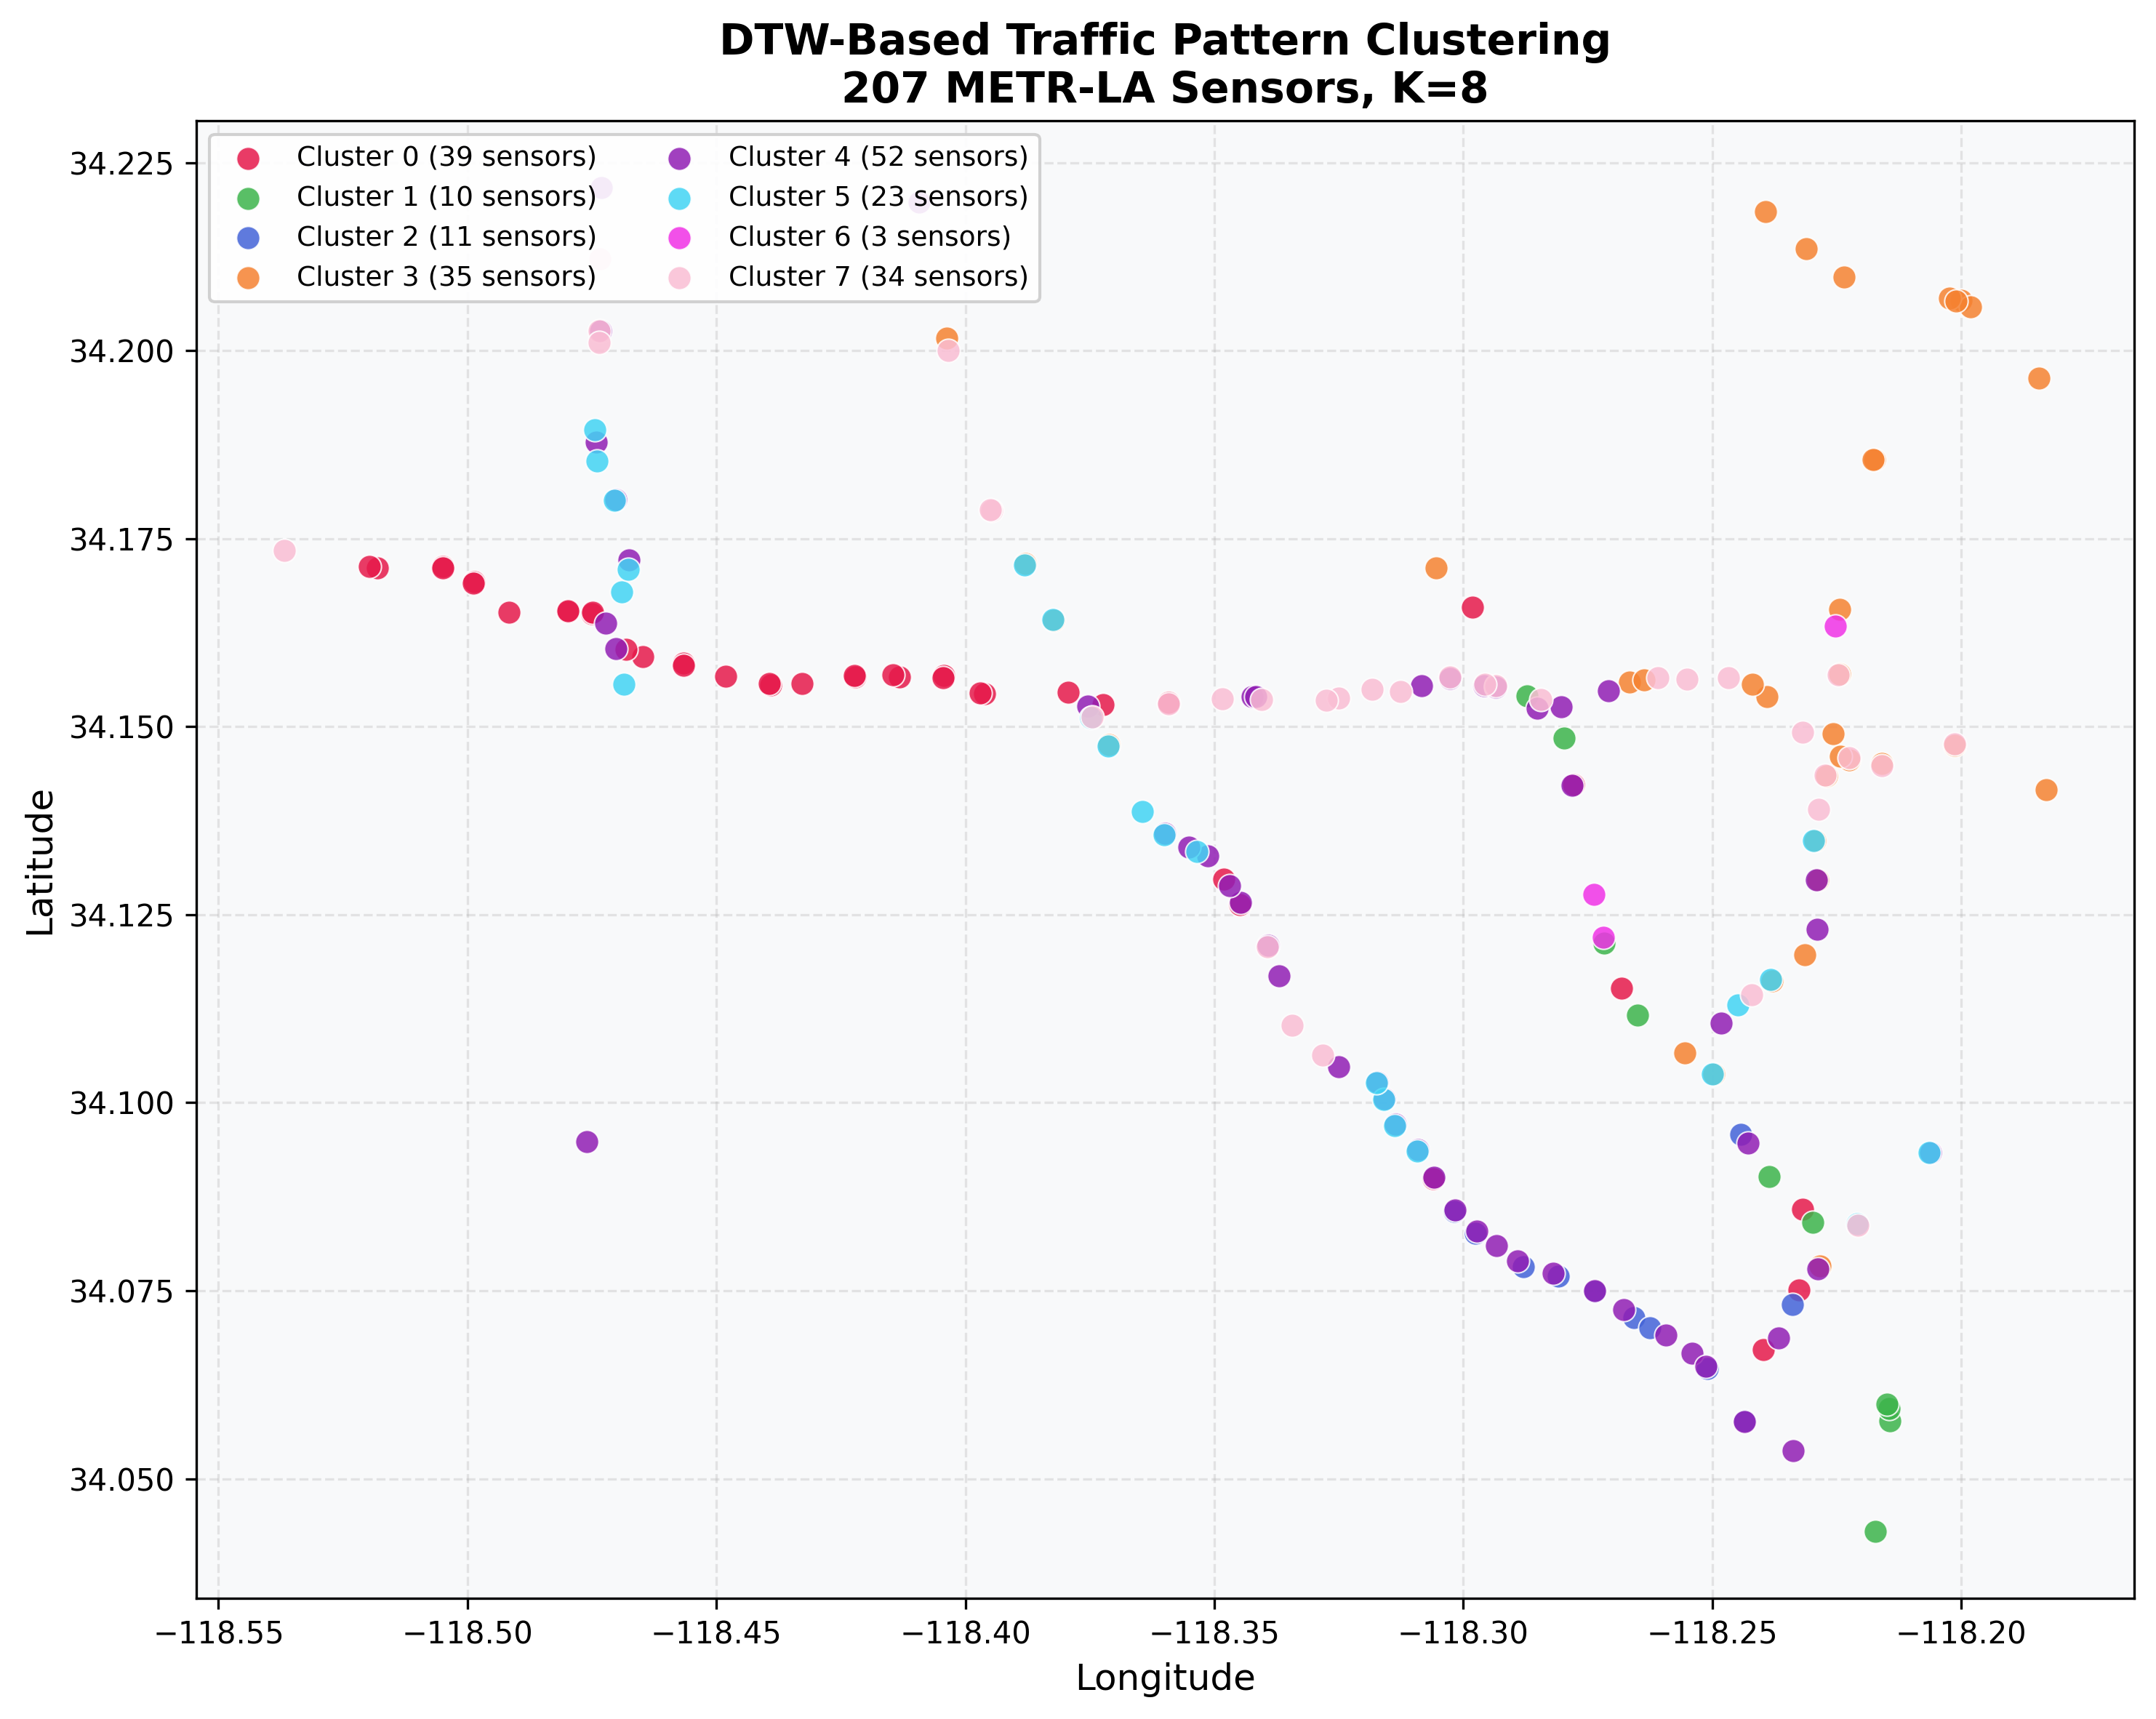
\includegraphics[width=\textwidth]{figures/dtw_clusters_map.png}
\caption{Geographic distribution of 207 METR-LA sensors colored by DTW cluster
assignment (K=8). Sensors in the same cluster share similar temporal traffic patterns
but are not necessarily geographically adjacent.}
\label{fig:dtw_distribution}
\end{figure}

\section{Local Model Architecture: GRU Encoder-Decoder}

Each client (sensor) trains a GRU-based Encoder-Decoder (Seq2Seq) model, following the architecture from Zhu et al. \cite{zhu2025cmba}. Building on the GRU and Seq2Seq foundations described in Section~\ref{sec:gru_theory}, this section details the specific architectural choices. While recent centralized approaches achieve strong performance with graph neural networks \cite{li2018, wu2019graphwavenet} or Transformers \cite{shuai2025fedtformer}, these architectures incur significantly larger parameter counts and communication costs when deployed in federated settings. Linear models such as Ridge regression are strong short-horizon baselines due to traffic autocorrelation (see Section~\ref{sec:stat_baselines}), but the GRU Seq2Seq backbone provides better long-horizon forecasting and lower RMSE while remaining lightweight (316K parameters, 1.26~MB per transfer). The design emphasis is therefore on the \textit{FL orchestration layer}, hierarchical aggregation, quality weighting, and adaptive selection, rather than on backbone complexity.

\label{sec:model}
\begin{figure}[htbp]
\centering
\includegraphics[width=\textwidth]{figures/gru_seq2seq.png}
\caption{GRU Encoder-Decoder (Seq2Seq) architecture used as the local model.}
\label{fig:gru_model}
\end{figure}
\subsection{Encoder}
The encoder is a multi-layer Gated Recurrent Unit (GRU) \cite{cho2014} that reads the input sequence $\mathbf{X} = [\mathbf{x}^{(1)}, \dots, \mathbf{x}^{(L)}]$ and produces a context hidden state $\mathbf{h}_c$ that summarizes the temporal patterns. Each GRU cell computes:
\begin{equation}
\mathbf{z}_t = \sigma(\mathbf{W}_z [\mathbf{h}_{t-1}, \mathbf{x}_t] + \mathbf{b}_z) \quad \text{(update gate)}
\end{equation}
\begin{equation}
\mathbf{r}_t = \sigma(\mathbf{W}_r [\mathbf{h}_{t-1}, \mathbf{x}_t] + \mathbf{b}_r) \quad \text{(reset gate)}
\end{equation}
\begin{equation}
\tilde{\mathbf{h}}_t = \tanh(\mathbf{W}_h [\mathbf{r}_t \odot \mathbf{h}_{t-1}, \mathbf{x}_t] + \mathbf{b}_h)
\end{equation}
\begin{equation}
\mathbf{h}_t = (1 - \mathbf{z}_t) \odot \mathbf{h}_{t-1} + \mathbf{z}_t \odot \tilde{\mathbf{h}}_t
\end{equation}
where $\sigma$ is the sigmoid function and $\odot$ denotes element-wise multiplication. The encoder uses $N_\ell = 2$ stacked GRU layers with hidden size $d_h = 128$ and inter-layer dropout $p = 0.2$. It accepts either univariate input (speed only, $d_{\text{in}} = 1$) or multivariate input with time-of-day features ($d_{\text{in}} = 3$).

\subsection{Decoder}
The decoder generates predictions autoregressively \cite{cho2014}, one step at a time. It receives the encoder's final hidden state $\mathbf{h}_c$ as its initial state and operates as:
\begin{equation}
\mathbf{h}_t^{\text{dec}}, \hat{y}_t = \text{DecoderStep}(\hat{y}_{t-1}, \mathbf{h}_{t-1}^{\text{dec}})
\end{equation}
where $\hat{y}_0 = x^{(L)}$ (the last observed speed value) and $\mathbf{h}_0^{\text{dec}} = \mathbf{h}_c$. The decoder GRU always has an input size of 1 (speed only), since only speed is predicted, time-of-day features are not propagated through the decoder. Each hidden state is projected to a scalar prediction through a two-layer fully connected network:
\begin{equation}
\hat{y}_t = \mathbf{W}_2 \cdot \text{ReLU}(\mathbf{W}_1 \mathbf{h}_t^{\text{dec}} + \mathbf{b}_1) + \mathbf{b}_2
\end{equation}
The decoder uses the same hidden size ($d_h = 128$) and number of layers ($N_\ell = 2$) as the encoder.

\subsection{Teacher Forcing}
% \label{sec:teacher_forcing}
% During training, autoregressive decoders can suffer from \textit{exposure bias}: errors in early predictions compound through subsequent steps. Teacher forcing \cite{williams1989} mitigates this by randomly replacing the model's own prediction with the ground-truth value at each decoder step. Although the implementation supports teacher forcing with configurable linear decay, the final experiments set the teacher forcing ratio to $p_{\text{tf}}=0.0$, so the decoder is trained fully autoregressively from the beginning. This matches the inference setting, where future ground-truth values are unavailable.

% \subsection{Model Configuration}
% Table~\ref{tab:model_config} summarizes the hyperparameters used throughout all experiments.

% \begin{table}[h]
% \centering
% \caption{Model and training hyperparameters.}
% \label{tab:model_config}
% \begin{tabular}{ll}
% \hline
% \textbf{Parameter} & \textbf{Value} \\
% \hline
% Encoder input size & 1 (speed) or 3 (speed + sin/cos ToD) \\
% Hidden size ($d_h$) & 128 \\
% GRU layers ($N_\ell$) & 2 \\
% Dropout ($p$) & 0.2 \\
% Sequence length ($L$) & 12 (1 hour) \\
% Forecast horizon ($H$) & 12 (1 hour) \\
% Learning rate & $5 \times 10^{-4}$ (Adam \cite{kingma2015adam}) \\
% Weight decay & $10^{-5}$ \\
% Batch size (train / eval) & 512 / 256 \\
% Gradient clipping & $\|\nabla\|_{\max} = 5.0$ \\
% Loss function & Mean Squared Error (MSE) \\
% Teacher forcing & $p_{\text{tf}} = 0.0$ (disabled) \\
% \hline
% \end{tabular}
% \end{table}

% Table~\ref{tab:fl_config} lists the federated training configuration used in the final experiments.

% \begin{table}[H]
% \centering
% \caption{Federated training configuration.}
% \label{tab:fl_config}
% \begin{tabular}{ll}
% \hline
% \textbf{Parameter} & \textbf{Value} \\
% \hline
% Communication rounds ($R$) & 60 \\
% Local optimization steps ($E$) & 20 \\
% Client selection & Adaptive reliability-based \\
% Average participation rate & $\approx$75\% \\
% Quality temperature ($\tau$) & 0.5 \\
% Hierarchical sync period ($P$) & 5 rounds \\
% Mixing coefficient ($\alpha$) & 0.9 \\
% Hierarchical weighting & DTW-distance weighted \\
% Learning rate schedule & $5{\times}10^{-4} \xrightarrow{r=40} 2.5{\times}10^{-4} \xrightarrow{r=50} 10^{-4}$ \\
% \hline
% \end{tabular}
% \end{table}

During autoregressive decoding, early prediction errors may compound across later forecast steps. Although the implementation supports teacher forcing \cite{williams1989}, the final experiments disable it by setting $p_{\text{tf}}=0.0$, so the decoder is trained fully autoregressively from the beginning. This matches the inference setting, where future ground-truth values are unavailable. All model hyperparameters are detailed in Chapter~\ref{ch:implementation}.



\section{Hierarchical Federated Learning Framework}
\label{sec:fl_framework}

The proposed framework implements a two-level aggregation strategy that balances \textit{intra-cluster specialization} with \textit{inter-cluster generalization}, inspired by multilevel FL architectures such as MFVSTGNN \cite{liu2023mfvstgnn} and FedTFormer \cite{shuai2025fedtformer}. Unlike these approaches, which employ heavyweight graph or Transformer backbones, the proposed framework pairs the lightweight GRU Seq2Seq model with DTW-weighted inter-cluster knowledge sharing. Algorithm~\ref{alg:hfl} provides the complete pseudocode.

\subsection{Level 1: Intra-Cluster Federated Averaging}
Within each cluster $\mathcal{C}_k$ ($k = 1, \dots, K$), the standard FedAvg protocol \cite{mcmahan2017} is executed. At each communication round $r$:

\textbf{(a) Model Broadcast.} The cluster model $\theta_k^{(r)}$ is broadcast to all sensors in $\mathcal{C}_k$.

\textbf{(b) Client Selection.} A subset $\mathcal{S}_k^{(r)} \subseteq \mathcal{C}_k$ of clients is selected to participate (see Section~\ref{sec:client_selection}).

\textbf{(c) Local Training.} Each selected client $i \in \mathcal{S}_k^{(r)}$ initializes its model with $\theta_k^{(r)}$ and performs $E$ local optimization steps on its private dataset $\mathcal{D}_i$.

\textbf{(d) Quality-Weighted Aggregation.} The updated local models are aggregated using quality-weighted FedAvg \cite{dai2024}:
\begin{equation}
\label{eq:qw_fedavg}
\theta_k^{(r+1)} = \sum_{i \in \mathcal{S}_k^{(r)}} w_i \cdot \theta_i^{(r)}, \quad w_i = \frac{\frac{n_i}{n_{\text{total}}} \cdot \exp(-\ell_i / \tau)}{\sum_{j \in \mathcal{S}_k^{(r)}} \frac{n_j}{n_{\text{total}}} \cdot \exp(-\ell_j / \tau)}
\end{equation}
where $n_i$ is the number of training samples for client $i$, $\ell_i$ is the average training loss achieved in round $r$, and $\tau = 0.5$ is a temperature parameter. This weighting scheme assigns higher influence to clients that achieve lower training loss, used as a heuristic proxy for update reliability. When $\tau \to \infty$, Equation~\ref{eq:qw_fedavg} reduces to standard sample-weighted FedAvg. It should be noted that lower local loss may also reflect easier or less variable local data rather than universally better update quality; the limitation of this heuristic is discussed in Section~\ref{sec:discussion}.


\subsection{Level 2: Inter-Cluster Hierarchical Aggregation}
\label{sec:hier_agg}
Every $P$ rounds (default $P = 5$), the cluster models exchange knowledge through a distance-weighted blending step. For each cluster $k$:
\begin{equation}
\label{eq:hier_blend}
\theta_k \leftarrow \alpha \cdot \theta_k + (1 - \alpha) \cdot \sum_{j \neq k} \omega_{kj} \cdot \theta_j
\end{equation}
where $\alpha \in [0, 1]$ is the mixing coefficient. In the final configuration, $\alpha = 0.9$, preserving 90\% of the cluster-specific model while incorporating 10\% DTW-weighted knowledge from other clusters. $\omega_{kj}$ are normalized inter-cluster weights defined below.

\textbf{DTW-Based Weighting.} To ensure that knowledge sharing is proportional to traffic pattern similarity (consistent with the DTW clustering), the inter-cluster weights are computed from the DTW distances between cluster-mean time series:
\begin{equation}
\omega_{kj} = \frac{1/\text{DTW}(\bar{\mathbf{s}}_k, \bar{\mathbf{s}}_j)}{\sum_{m \neq k} 1/\text{DTW}(\bar{\mathbf{s}}_k, \bar{\mathbf{s}}_m)}
\end{equation}
where $\bar{\mathbf{s}}_k$ is the average time series of all sensors in cluster $k$. This means clusters with similar traffic dynamics share more model knowledge, while dissimilar clusters are largely independent.

The hierarchical synchronization is \textit{skipped on the final round} to prevent corruption of the converged model with no subsequent training rounds to recover.

\textbf{Geographic Weighting (Baseline).} As a comparison, the framework also supports geographic distance-based weighting, where $\omega_{kj}$ is computed using inverse Haversine distances between cluster centroids rather than DTW distances.

\subsection{Adaptive Client Selection}
\label{sec:client_selection}
In realistic edge networks, client availability is dynamic due to intermittent connectivity, variable computational load, and bandwidth constraints \cite{nishio2019, lai2021oort}. The framework models these conditions and implements adaptive selection.

\subsubsection{Network Condition Simulation}
% Each sensor $i$ is assigned a fixed \textit{reliability profile} drawn from one of three tiers, summarized in Table~\ref{tab:client_profiles}. Here $p_i$ is the Bernoulli availability probability and $\lambda_i$ is the expected communication latency.

% \begin{table}[H]
% \centering
% \caption{Simulated client reliability profiles.}
% \label{tab:client_profiles}
% \begin{tabular}{llll}
% \hline
% \textbf{Tier} & \textbf{Share} & \textbf{Availability $p_i$} & \textbf{Latency $\lambda_i$} \\
% \hline
% Stable & 60\% & $\mathcal{U}(0.85, 0.95)$ & $\mathcal{U}(50, 150)$ ms \\
% Moderate & 25\% & $\mathcal{U}(0.55, 0.70)$ & $\mathcal{U}(150, 350)$ ms \\
% Unreliable & 15\% & $\mathcal{U}(0.20, 0.40)$ & $\mathcal{U}(350, 500)$ ms \\
% \hline
% \end{tabular}
% \end{table}
Each sensor $i$ is assigned a fixed \textit{reliability profile} drawn from one of three tiers (Stable, Moderate, Unreliable), with varying availability probabilities and communication latencies. The specific tier distributions are detailed in Chapter~\ref{ch:implementation}.

\subsubsection{Reliability Score}
A composite reliability score combines availability and latency into a single metric:
\begin{equation}
\label{eq:reliability}
s_i = p_i \cdot \exp\left(-\frac{\lambda_i}{\lambda_{\max}}\right)
\end{equation}
where $\lambda_{\max} = 500$ ms is the normalization ceiling. Higher scores indicate more reliable clients.

\subsubsection{Selection Strategies}
The framework implements three selection strategies for ablation comparison:
\begin{enumerate}
    \item \textbf{Full Participation:} All clients in the cluster train every round ($|\mathcal{S}_k| = |\mathcal{C}_k|$). Used as the upper-bound baseline.
    \item \textbf{Random Dropout:} Each client is available with probability $p_i$ (Bernoulli sampling). Surviving clients are selected in random order. Models the uncontrolled dynamic case.
    \item \textbf{Adaptive Reliability:} Under the same Bernoulli dropout conditions, available clients are ranked by $s_i$ and the top-ranked clients are selected. To maintain a controlled minimum participation rate in the simulation, if the sampled available set falls below the 50\% floor, additional clients are selected according to reliability scores. This floor represents a controlled experimental assumption rather than a real-world guarantee of availability.
\end{enumerate}

\subsection{Communication Cost Model}
\label{sec:comm_cost}
The total communication cost per FL round is computed following the accounting framework of Zhu et al. \cite{zhu2025cmba}:
\begin{equation}
\label{eq:comm_cost}
C_{\text{round}} = \sum_{k=1}^{K} \left( |\mathcal{S}_k| \cdot B_{\text{up}} + |\mathcal{C}_k| \cdot B_{\text{down}} \right)
\end{equation}
where $B_{\text{up}}$ is the upload cost per client (model parameters in \texttt{float32}, 4 bytes each), and $B_{\text{down}}$ is the download cost (full model broadcast to all cluster members). When hierarchical synchronization fires, an additional cost of $2K \cdot B_{\text{model}}$ is incurred for inter-cluster model exchange.
\subsection{Practical Deployment Model}
\label{sec:deployment}

In the experimental formulation, each sensor is treated as a logical FL client because each sensor stream has its own data distribution. In a real ITS deployment, however, raw loop-detector sensors cannot independently store historical data or perform model training. The physical training client is a Roadside Unit (RSU) or Multi-access Edge Computing (MEC) node \cite{nishio2019, bonawitz2019}. The deployment model consists of five layers:

\begin{enumerate}
    \item \textbf{Sensor layer:} Loop detectors and roadside sensors collect speed readings at 5-minute intervals and transmit them to the nearest RSU/MEC node as part of normal ITS sensing operations.
    \item \textbf{RSU/MEC edge layer:} Each RSU receives measurements from nearby sensors, stores rolling historical windows (approximately 5.5~MB per sensor for the training split), and performs local model training.
    \item \textbf{Logical clustering layer:} Each sensor stream is assigned to a DTW traffic-pattern cluster. This assignment is logical, not physical: a single RSU may host sensors belonging to multiple DTW clusters, and a single DTW cluster may include streams hosted by different RSUs.
    % \item \textbf{Cluster aggregation layer:} A regional server aggregates model updates from all edge devices within each cluster.
    % \item \textbf{City/cloud orchestration layer:} A central coordination server manages communication rounds and inter-cluster hierarchical synchronization.
\end{enumerate}

It is important to distinguish the physical assignment from the logical assignment. Geographic assignment determines which RSU receives the sensor stream; DTW clustering determines which cluster model the stream contributes to during federated training. For example, if RSU~A receives data from sensors~1, 2, 3, and 4, but sensor~1 belongs to DTW Cluster~0 while sensor~2 belongs to DTW Cluster~3, then RSU~A stores and trains separate local models $\theta_0$ and $\theta_3$, and participates in two cluster federations independently. This is architecturally straightforward because the computational load per client is small (316K parameters, 1.26~MB per transfer).

This setup does not introduce an additional repeated model-communication path. Sensors do not download models or upload gradients; they only provide measurements to their serving RSU, which is part of normal ITS sensing. The repeated FL communication remains model uploads and downloads between RSU/MEC nodes and aggregation servers, which is exactly what the communication cost model in Equation~(\ref{eq:comm_cost}) measures.

\subsection{Communication Cost Decomposition}
\label{sec:comm_decomp}

To clarify what the reported communication cost includes and excludes, the total network traffic in the deployment can be decomposed as:
\begin{equation}
\label{eq:comm_decomp}
C_{\text{total}} = C_{\text{sensing}} + C_{\text{init}} + C_{\text{FL}} + C_{\text{control}}
\end{equation}
where:
\begin{itemize}
    \item $C_{\text{sensing}}$ is operational sensor-to-RSU measurement reporting (approximately 238~KB/day for 207 sensors at 5-minute intervals). This cost exists in both centralized and federated ITS deployments and is not counted.
    \item $C_{\text{init}}$ is the one-time DTW clustering initialization overhead: transmitting short representative sequences ($207 \times 300 \times 4$~bytes $\approx$ 0.24~MB). This is negligible and reported separately.
    \item $C_{\text{FL}}$ is the repeated FL model-training communication: model downloads, client uploads, and hierarchical synchronization. This is the cost reported throughout this thesis (21.5--25.8~GB).
    \item $C_{\text{control}}$ is metadata traffic for cluster labels, selection decisions, and availability flags, which is negligible.
\end{itemize}

The reported communication cost of 21.5--25.8~GB therefore measures $C_{\text{FL}}$ only. It does not include operational sensor-to-RSU reporting, and it does not represent total ITS network traffic. The RSU/MEC deployment clarification changes the physical endpoint of training but does not add a new repeated model-communication path.

\subsection{Algorithm Summary}

\begin{algorithm}[H]
\caption{Hierarchical Federated Learning for Traffic Prediction}
\label{alg:hfl}
\begin{algorithmic}[1]
\REQUIRE Sensor clusters $\{\mathcal{C}_1, \dots, \mathcal{C}_K\}$ via DTW, initial model $\theta^{(0)}$, rounds $R$, local optimization steps $E$, mixing coefficient $\alpha$, sync period $P$, LR schedule
\STATE Initialize all cluster models: $\theta_k^{(0)} \leftarrow \theta^{(0)}$ for $k = 1, \dots, K$
\FOR{$r = 1$ to $R$}
    \STATE Update learning rate if $r$ matches a schedule milestone
    \FOR{each cluster $k = 1, \dots, K$}
        \STATE Broadcast $\theta_k^{(r-1)}$ to all clients in $\mathcal{C}_k$
        \STATE $\mathcal{S}_k \leftarrow \textsc{SelectClients}(\mathcal{C}_k)$ \COMMENT{Adaptive selection}
        \FOR{each client $i \in \mathcal{S}_k$ \textbf{in parallel}}
            \STATE $\theta_i \leftarrow \textsc{LocalTrain}(\theta_k^{(r-1)}, \mathcal{D}_i, E)$
        \ENDFOR
        \STATE $\theta_k^{(r)} \leftarrow \textsc{QualityWeightedAvg}(\{\theta_i\}_{i \in \mathcal{S}_k})$ \COMMENT{Level 1}
    \ENDFOR
    \IF{$r \bmod P = 0$ \AND $r < R$}
        \FOR{each cluster $k$}
            \STATE $\theta_k^{(r)} \leftarrow \alpha \cdot \theta_k^{(r)} + (1 - \alpha) \sum_{j \neq k} \omega_{kj} \theta_j^{(r)}$ \COMMENT{Level 2}
        \ENDFOR
    \ENDIF
\ENDFOR
\RETURN $\{\theta_1^{(R)}, \dots, \theta_K^{(R)}\}$
\end{algorithmic}
\end{algorithm}

% \section{Evaluation Metrics}
% \label{sec:metrics}

% Model performance is evaluated using three standard traffic forecasting metrics \cite{li2018}, computed on denormalized predictions in original speed units (mph):

% \textbf{Mean Absolute Error (MAE):}
% \begin{equation}
% \text{MAE} = \frac{1}{n} \sum_{i=1}^{n} |y_i - \hat{y}_i|
% \end{equation}

% \textbf{Root Mean Squared Error (RMSE):}
% \begin{equation}
% \text{RMSE} = \sqrt{\frac{1}{n} \sum_{i=1}^{n} (y_i - \hat{y}_i)^2}
% \end{equation}

% \textbf{Mean Absolute Percentage Error (MAPE):}
% \begin{equation}
% \text{MAPE} = \frac{100\%}{|\mathcal{M}|} \sum_{i \in \mathcal{M}} \left|\frac{y_i - \hat{y}_i}{y_i}\right|
% \end{equation}
% where $\mathcal{M} = \{i : |y_i| > 5.0\}$ masks out near-zero speed values where percentage error is undefined, following the convention established by Li et al. \cite{li2018}.

% All metrics are reported both as overall averages across all sensors and all horizons, and disaggregated by prediction horizon (15, 30, and 60 minutes) to analyze how prediction quality degrades with increasing forecast distance.
